\documentclass{article}
\usepackage[english]{babel}
\usepackage[utf8]{inputenc}
\usepackage[T1]{fontenc}
\usepackage{amsmath}
\usepackage[us]{datetime}
\usepackage{graphicx}
\usepackage[font=small,labelfont=bf]{caption}
\usepackage[font=small,labelfont=bf]{subcaption}
\usepackage{listings}
\usepackage{color}
\renewcommand{\lstlistingname}{Code}
\captionsetup[subfigure]{font=footnotesize}
\setlength{\parindent}{0in}


\author{Madis Ollikainen}
\title{Progress report: No Wealth Accumulation (NWA)}

\begin{document}

\maketitle

%% For Stefanos comments %% 
%\section{Stefano's comment}
%{\color{red}I will write my comments in red, so that you can spot them easily.}

I implemented codes for both Nash eq. and simple learning simulations, in which the maximum contribution is fixed to a $W_0$ given in the \emph{config.conf} file. Thus the grouping methods 1 and 3, as well as 2 and 4 became pairwise equivalent. Nevertheless at the moment I still simulated all of the grouping methods just to check the code. 

I some small sized ensemble simulations, with ensemble size being $NE = 10$ societies and each society having $N = 500$ players during $T = 100$ time steps. On figure 1 you'll see the comparison of Nash eq. simulations and simple learning simulations for equal talent (and no wealth accumulation). And on figures 2-4 you'll see a small parameter sweep for the beta parameter in the simple learning simulations. The beta parameter was ranged in $\beta = {0.05, 0.25, 0.5, 0.75, 1.0}$.

I guess I might run some longer control simulations for the equal talent case. Maybe up to a $T = 200$ or so time steps, to see if something interesting happens later. This parametric sweep for beta was just a test. I think I should also look into larger beta values.  

Interestingly, even though the grouping schemas 1\&3 should give equivalent result, the main difference seen for the beta sweep for different betas is the change in the difference between gini coefficient for these two cases. I guess I still have to check trough the code and conduct some extra test runs (with different $W_0$ for example, at the moment I used $W_0=2.0$). Could this be a result of the sorting algorithm you used? 

%% Equal talen %% 
\begin{figure}[h]
\centering

% Nash equlibrim eq. talent %

\begin{subfigure}[t]{0.38\textwidth}
\centering
\includegraphics[width=\textwidth]{{nashEQ_eqTal_NWA_combined/cooperation}.pdf}
\caption{Cooperation (Nash eq.) }
\end{subfigure}%
%
\hfill
%
\begin{subfigure}[t]{0.38\textwidth}
\centering
\includegraphics[width=\textwidth]{{sml_eqTal_NWA_combined/cooperation}.pdf}
\caption{Cooperation (Simple Learning) }
\end{subfigure}%
%
\bigskip 
%

\begin{subfigure}[t]{0.38\textwidth}
\centering
\includegraphics[width=\textwidth]{{nashEQ_eqTal_NWA_combined/gini}.pdf}
\caption{Gini (Nash eq.) }
\end{subfigure}%
%
\hfill
%
\begin{subfigure}[t]{0.38\textwidth}
\centering
\includegraphics[width=\textwidth]{{sml_eqTal_NWA_combined/gini}.pdf}
\caption{Gini (Simple Learning) }
\end{subfigure}%
%
\bigskip 
%

\begin{subfigure}[t]{0.38\textwidth}
\centering
\includegraphics[width=\textwidth]{{nashEQ_eqTal_NWA_combined/wealth}.pdf}
\caption{Total wealth (Nash eq.) }
\end{subfigure}%
%
\hfill
%
\begin{subfigure}[t]{0.38\textwidth}
\centering
\includegraphics[width=\textwidth]{{sml_eqTal_NWA_combined/wealth}.pdf}
\caption{Total wealth (Simple Learning) }
\end{subfigure}%
%
\bigskip 
%



\begin{subfigure}[t]{0.38\textwidth}
\centering
\includegraphics[width=\textwidth]{{nashEQ_eqTal_NWA_combined/efficiency}.pdf}
\caption{Efficiency (Nash eq.) }
\end{subfigure}%
%
\hfill
%
\begin{subfigure}[t]{0.38\textwidth}
\centering
\includegraphics[width=\textwidth]{{sml_eqTal_NWA_combined/efficiency}.pdf}
\caption{Efficiency (Simple Learning) }
\end{subfigure}%
%
\bigskip 
%

\bigskip

\caption{Comparison of Nash eq. and simple learning simulations with no wealth accumulations and equal talent for all agents. NOTE: as both $w_i$ and $r_i$ are equal for all the agents, all of the grouping methods should give the same results, which is also seen on the plots. Number of agents $N = 500$, size of ensemble $NE = 10$, simulation duration $T = 100$, beta $\beta = 0.05$, learning parameter $\xi = 0.1$.}
\end{figure}

\break

\begin{figure}[h]
\centering

% Cooperation %

\begin{subfigure}[t]{0.33\textwidth}
\centering
\includegraphics[width=\textwidth]{{sml_NWA_beta_0.05_combined/cooperation}.pdf}
\caption{Cooperation ($\beta = 0.05$) }
\end{subfigure}%
%
\hfill
%
\begin{subfigure}[t]{0.33\textwidth}
\centering
\includegraphics[width=\textwidth]{{sml_NWA_beta_0.25_combined/cooperation}.pdf}
\caption{Cooperation ($\beta = 0.25$) }
\end{subfigure}%
%
\hfill
%
\begin{subfigure}[t]{0.33\textwidth}
\centering
\includegraphics[width=\textwidth]{{sml_NWA_beta_0.5_combined/cooperation}.pdf}
\caption{Cooperation ($\beta = 0.5$) }
\end{subfigure}%
%
\hfill
%
\bigskip
\begin{subfigure}[c]{0.33\textwidth}
\centering
\includegraphics[width=\textwidth]{{sml_NWA_beta_0.75_combined/cooperation}.pdf}
\caption{Cooperation ($\beta = 0.75$) }
\end{subfigure}%
%
\hfill
%
\begin{subfigure}[c]{0.33\textwidth}
\centering
\includegraphics[width=\textwidth]{{sml_NWA_beta_1.0_combined/cooperation}.pdf}
\caption{Cooperation ($\beta = 1 $) }
\end{subfigure}%
%
\hfill
%
\begin{subfigure}[c]{0.33\textwidth}
\centering
\includegraphics[width=\textwidth]{{sml_NWA_beta_2.0_combined/cooperation}.pdf}
\caption{Cooperation ($\beta = 2 $) }
\end{subfigure}%
%
\hfill
%

\caption{Cooperation in beta scan for simple learning. NOTE: as $w_i$ is equal for all the agents, grouping schemas 1\&3 and 2\&4 should give same (similar) results. Number of agents $N = 500$, size of ensemble $NE = 10$, simulation duration $T = 100$, learning parameter $\xi = 0.1$.}
\end{figure}




\begin{figure}[h]
\centering

% Gini %

\begin{subfigure}[t]{0.33\textwidth}
\centering
\includegraphics[width=\textwidth]{{sml_NWA_beta_0.05_combined/gini}.pdf}
\caption{Gini ($\beta = 0.05$) }
\end{subfigure}%
%
\hfill
%
\begin{subfigure}[t]{0.33\textwidth}
\centering
\includegraphics[width=\textwidth]{{sml_NWA_beta_0.25_combined/gini}.pdf}
\caption{Gini ($\beta = 0.25$) }
\end{subfigure}%
%
\hfill
%
\begin{subfigure}[t]{0.33\textwidth}
\centering
\includegraphics[width=\textwidth]{{sml_NWA_beta_0.5_combined/gini}.pdf}
\caption{Gini ($\beta = 0.5$) }
\end{subfigure}%
%
\hfill
%
\bigskip
\begin{subfigure}[c]{0.33\textwidth}
\centering
\includegraphics[width=\textwidth]{{sml_NWA_beta_0.75_combined/gini}.pdf}
\caption{Gini ($\beta = 0.75$) }
\end{subfigure}%
%
\hfill
%
\begin{subfigure}[c]{0.33\textwidth}
\centering
\includegraphics[width=\textwidth]{{sml_NWA_beta_1.0_combined/gini}.pdf}
\caption{Gini ($\beta = 1 $) }
\end{subfigure}%
%
\hfill
%
\begin{subfigure}[c]{0.33\textwidth}
\centering
\includegraphics[width=\textwidth]{{sml_NWA_beta_2.0_combined/gini}.pdf}
\caption{Gini ($\beta = 2 $) }
\end{subfigure}%
%
\hfill
%

\caption{Gini coef. in beta scan for simple learning. NOTE: as $w_i$ is equal for all the agents, grouping schemas 1\&3 and 2\&4 should give same (similar) results. Number of agents $N = 500$, size of ensemble $NE = 10$, simulation duration $T = 100$, learning parameter $\xi = 0.1$.}
\end{figure}



\begin{figure}[h]
\centering

% Gini %

\begin{subfigure}[t]{0.33\textwidth}
\centering
\includegraphics[width=\textwidth]{{sml_NWA_beta_0.05_combined/wealth}.pdf}
\caption{Wealth ($\beta = 0.05$) }
\end{subfigure}%
%
\hfill
%
\begin{subfigure}[t]{0.33\textwidth}
\centering
\includegraphics[width=\textwidth]{{sml_NWA_beta_0.25_combined/wealth}.pdf}
\caption{Wealth ($\beta = 0.25$) }
\end{subfigure}%
%
\hfill
%
\begin{subfigure}[t]{0.33\textwidth}
\centering
\includegraphics[width=\textwidth]{{sml_NWA_beta_0.5_combined/wealth}.pdf}
\caption{Wealth ($\beta = 0.5$) }
\end{subfigure}%
%
\hfill
%
\bigskip
\begin{subfigure}[c]{0.33\textwidth}
\centering
\includegraphics[width=\textwidth]{{sml_NWA_beta_0.75_combined/wealth}.pdf}
\caption{Wealth ($\beta = 0.75$) }
\end{subfigure}%
%
\hfill
%
\begin{subfigure}[c]{0.33\textwidth}
\centering
\includegraphics[width=\textwidth]{{sml_NWA_beta_1.0_combined/wealth}.pdf}
\caption{Wealth ($\beta = 1 $) }
\end{subfigure}%
%
\hfill
%
\begin{subfigure}[c]{0.33\textwidth}
\centering
\includegraphics[width=\textwidth]{{sml_NWA_beta_2.0_combined/wealth}.pdf}
\caption{Wealth ($\beta = 2 $) }
\end{subfigure}%
%
\hfill
%

\caption{Total wealth in beta scan for simple learning. NOTE: as $w_i$ is equal for all the agents, grouping schemas 1\&3 and 2\&4 should give same (similar) results. Number of agents $N = 500$, size of ensemble $NE = 10$, simulation duration $T = 100$, learning parameter $\xi = 0.1$.}
\end{figure}






\begin{figure}[h]
\centering

% Gini %

\begin{subfigure}[t]{0.33\textwidth}
\centering
\includegraphics[width=\textwidth]{{sml_NWA_beta_0.05_combined/efficiency}.pdf}
\caption{Efficiency ($\beta = 0.05$) }
\end{subfigure}%
%
\hfill
%
\begin{subfigure}[t]{0.33\textwidth}
\centering
\includegraphics[width=\textwidth]{{sml_NWA_beta_0.25_combined/efficiency}.pdf}
\caption{Efficiency ($\beta = 0.25$) }
\end{subfigure}%
%
\hfill
%
\begin{subfigure}[t]{0.33\textwidth}
\centering
\includegraphics[width=\textwidth]{{sml_NWA_beta_0.5_combined/efficiency}.pdf}
\caption{Efficiency ($\beta = 0.5$) }
\end{subfigure}%
%
\hfill
%
\bigskip
\begin{subfigure}[c]{0.33\textwidth}
\centering
\includegraphics[width=\textwidth]{{sml_NWA_beta_0.75_combined/efficiency}.pdf}
\caption{Efficiency ($\beta = 0.75$) }
\end{subfigure}%
%
\hfill
%
\begin{subfigure}[c]{0.33\textwidth}
\centering
\includegraphics[width=\textwidth]{{sml_NWA_beta_1.0_combined/efficiency}.pdf}
\caption{Efficiency ($\beta = 1 $) }
\end{subfigure}%
%
\hfill
%
\begin{subfigure}[c]{0.33\textwidth}
\centering
\includegraphics[width=\textwidth]{{sml_NWA_beta_2.0_combined/efficiency}.pdf}
\caption{Efficiency ($\beta = 2 $) }
\end{subfigure}%
%
\hfill
%

\caption{Efficiency in beta scan for simple learning. NOTE: as $w_i$ is equal for all the agents, grouping schemas 1\&3 and 2\&4 should give same (similar) results. Number of agents $N = 500$, size of ensemble $NE = 10$, simulation duration $T = 100$, learning parameter $\xi = 0.1$.}
\end{figure}



\end{document}